\chapter{MXNet}

参考文献:\href{https://mxnet.incubator.apache.org/architecture/index.html}{MXNet Architecture}

{\color{red}Time: 2018.05.18}

\section{Optimizing Memory Consumption in DL}
Over the last ten years, a constant trend in deep learning is towards deeper and larger networks. Despite rapid advances in hardware performance, cutting-edge deep learning models continue to push the limits of GPU RAM. So even today, it’s always desirable to find ways to train larger models while consuming less memory. Doing so enables us to train faster, using larger batch sizes, and consequently achieving a higher GPU utilization rate.

\subsection{Computation Graph}
A computation graph describes the (data flow) dependencies between the operations in the deep network. The operations performed in the graph can be either fine-grained or coarse-grained.

The concept of a computation graph is explicitly encoded in packages like Theano and CGT. In other libraries, computation graphs appear implicitly as network configuration files. The major difference in these libraries comes down to how they calculate gradients. There are mainly two ways: performing back-propagation on the same graph or explicitly representing a backwards path to calculate the required gradients.

\begin{figure}[!hbtp]
\centering
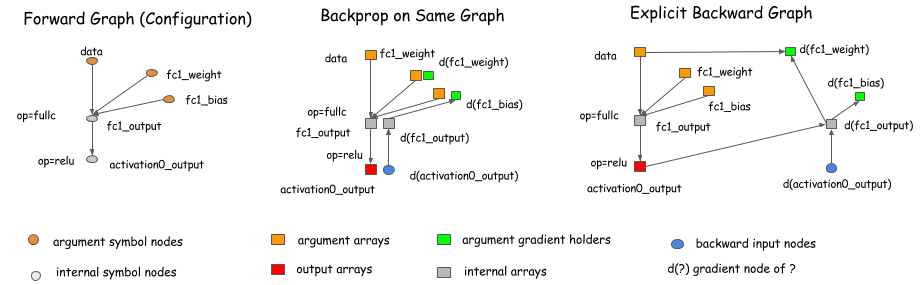
\includegraphics[width=0.85\textwidth]{MXNet/back_graph}
\caption{The implicitly \& explicitly back-propagation on Graph}
\end{figure}

Libraries like Caffe, CXXNet, and Torch take the former approach, performing back-prop on the original graph. Libraries like Theano and CGT take the latter approach, explicitly representing the backward path. In this discussion, we adopt the explicit backward path approach because it has several advantages for optimization.

We adopt the explicit backward path approach because it has several advantages for optimization.

Why is explicit backward path better? Two reasons:
\begin{itemize}
\item The explicit backward path clearly describes the dependency between computations.\\
Like the following case, where we want to get the gradient of \textbf{A} and \textbf{B}. As we can see clearly from the graph, the computation of the $d(C)$ gradient doesn’t depend on $F$. This means that we can free the memory of $F$ right after the forward computation is done. Similarly, the memory of $F$ can be recycled.
\begin{figure}[!hbtp]
\centering
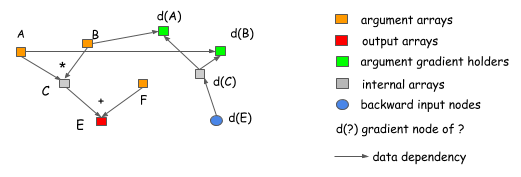
\includegraphics[width=0.85\textwidth]{MXNet/back_dep_prune}
\caption{Dependencies can be found quickly.}
\end{figure}

\item Another advantage of the explicit backward path is the ability to have a different backward path, instead of a mirror of forward one.\\
A common example is the split connectioncase, as shown in the following figure.
\begin{figure}[!hbtp]
\centering
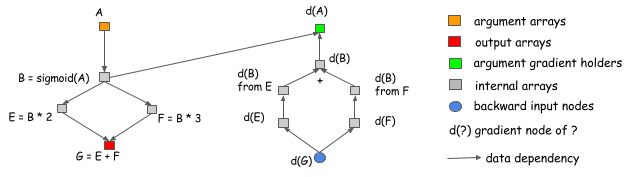
\includegraphics[width=0.85\textwidth]{MXNet/back_agg_grad}
\caption{Different backward path from forward path.}
\end{figure}
In this example, the output of \textbf{B} is referenced by two operations. If we want to do the gradient calculation in the same network, we need to introduce an explicit split layer. This means we need to do the split for the forward pass, too. In this figure, the forward pass doesn’t contain a split layer, but the graph will automatically insert a gradient aggregation node before passing the gradient back to \textbf{B}. This helps us to save the memory cost of allocating the output of the split layer, and the operation cost of replicating the data in the forward pass.
\end{itemize}

\subsection{What Can be Optimized?}
As you can see, the computation graph is a useful way to discuss memory allocation optimization techniques. Already, we’ve shown how you can save some memory by using the explicit backward graph. Now let’s explore further optimizations, and see how we might determine reasonable baselines for benchmarking.

Assume that we want to build a neural network with \textit{n} layers. Typically, when implementing a neural network, we need to allocate node space for both the output of each layer and the gradient values used during back-propagation. This means we need roughly $2n$ memory cells. We face the same requirement when using the explicit backward graph approach because the number of nodes in a backward pass is roughly the same as in a forward pass.

\subsubsection{In-place Operations}
One of the simplest techniques we can employ is \textit{In-place memory sharing} across operations. For neural networks, we can usually apply this technique for the operations corresponding to activation functions. 

''In-place'' means using same memory for input and output. But you should be careful about that the result is used by more than one operation! 

\subsubsection{Standard Memory Sharing}
In-place operations are not the only places where we can share memory. In the following example, because the value of B is no longer needed after we compute E, we can reuse B’s memory to hold the result of E.
\begin{figure}[!hbtp]
\centering
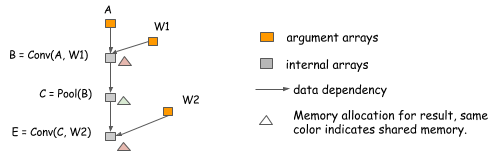
\includegraphics[width=0.85\textwidth]{MXNet/alloc_normal}
\caption{Standard Memory sharing between \textbf{B} \& the result of \textbf{E}.}
\end{figure}

Memory sharing doesn't necessarily require the same data shape. Note that in the preceding example, the shapes of \textbf{B} and \textbf{E} can differ. To handle such a situation, we can allocate a memory region of size equal to the maximum of that required by \textbf{B} and \textbf{E} and share it between them.

\subsection{Memory Allocation Algorithm}
Based on the '' In-Place Operatioins'', how can we allocate memory correctly?

The key problem is that we need to place resources so that they don’t conflict with each other. More specifically, each variable has a \textbf{life time} between the time it gets computed until the last time it is used. In the case of the multi-layer perceptron, the life time of \textit{fc1} ends after \textit{act1} get computed.
\index{Life Time}
See below figure:
\begin{figure}[!hbtp]
\centering
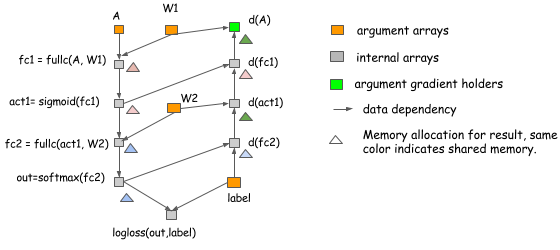
\includegraphics[width=0.85\textwidth]{MXNet/alloc_mlp}
\caption{Standard Memory sharing between \textbf{B} \& the result of \textbf{E}.}
\end{figure}

The principle is to allow memory sharing only between variables whose lifetimes don’t overlap. There are multiple ways to do this. You can construct the conflicting graph with each variable as a node and link the edge between variables with overlapping lifespans, and then run a graph-coloring algorithm. This likely has $O(n^2)$ complexity, where \textit{n} is the number of nodes in the graph. This might be too costly.

Let’s consider another simple heuristic. The idea is to simulate the procedure of traversing the graph, and keep a count of future operations that depends on the node.
\begin{figure}[!hbtp]
\centering
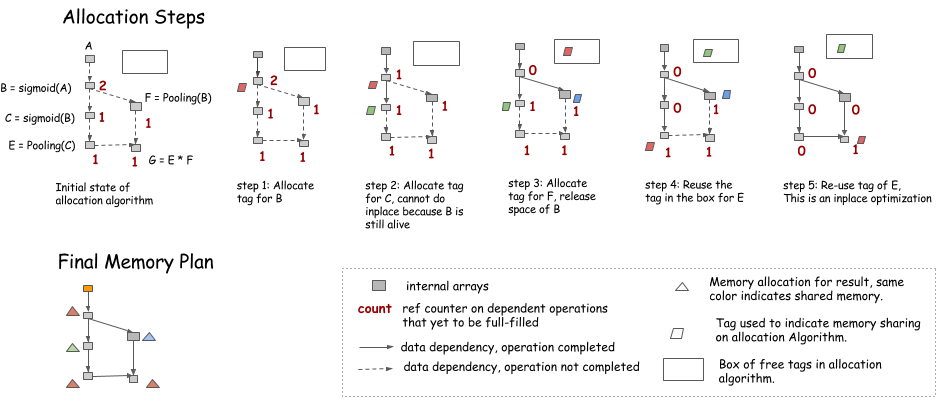
\includegraphics[width=0.95\textwidth]{MXNet/alloc_step}
\caption{Standard Memory sharing between \textbf{B} \& the result of \textbf{E}.}
\end{figure}
\begin{itemize}
\item An in-place optimization can be performed when only the current operation depends on the source (i.e. count == 1).
\item Memory can be recycled into the box on the upper right corner when the \textit{count} goes to 0.
\item When we need new memory, we can either get it from the box or allocate a new one. 
\end{itemize}

\textbf{Noet:} During the simulation, no memory is allocated. Instead, we keep a record of how much memory each node needs, and allocate the maximum of the shared parts in the final memory plan.

\subsection{Static vs. Dynamic Allocation}
The major difference is that static allocation is only done once, so we can afford to use more complicated algorithms. For example, we can search for memory sizes that are similar to the required memory block. The Allocation can also be made graph aware. We’ll talk about that in the next section. Dynamic allocation puts more pressure on fast memory allocation and garbage collection.

There is also one takeaway for users who want to rely on dynamic memory allocations: do not unnecessarily reference objects. For example, if we organize all of the nodes in a list and store then in a Net object, these nodes will never get dereferenced, and we gain no space. Unfortunately, this is a common way to organize code.

\subsection{Memory Allocation for Parallel Operations}
In the previous section, we discussed how we can simulate running the procedure for a computation graph to get a static allocation plan. However, optimizing for parallel computation presents other challenges because resource sharing and parallelization are on the two ends of a balance. Let’s look at the following two allocation plans for the same graph:
\begin{figure}[!hbtp]
\centering
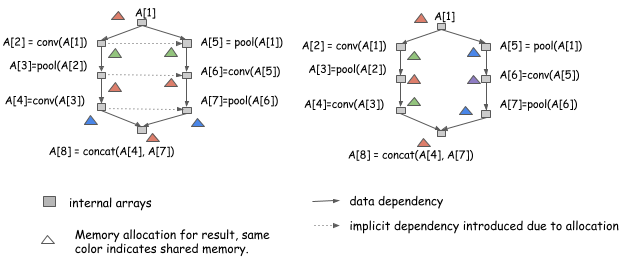
\includegraphics[width=0.95\textwidth]{MXNet/parallel_alloc}
\caption{Standard Memory sharing between \textbf{B} \& the result of \textbf{E}.}
\end{figure}

Both allocation plans are valid if we run the computation serially, {\bfseries from $A[1]$ to $A[8]$. } However, the allocation plan on the left introduces additional dependencies, which means we can't run computation of $A[2]$ and $A[5]$ in parallel. The plan on the right can. To parallelize computation, we need to take greater care. 

\subsubsection{Be Correct and Safe First}
Being correct is our first principle. This means to execute in a way that takes implicit dependency memory sharing into consideration. You can do this by adding the implicit dependency edge to the execution graph. Or, even simpler, if the execution engine is mutation aware, as described in \href{https://mxnet.incubator.apache.org/architecture/note_engine.html}{our discussion of dependency engine design}, push the operation in sequence and write to the same variable tag that represents the same memory region.

Always produce a safe memory allocation plan. This means never allocate the same memory to nodes that can be parallelized. This might not be ideal when memory reduction is more desirable, and we don’t gain too much when we can get benefit from multiple computing streams simultaneously executing on the same GPU.

\subsubsection{Try to Allow More Parallelization}
Now we can safely perform some optimizations. The general idea is to try and encourage memory sharing between nodes that can’t be parallelized. You can do this by creating an ancestor relationship graph and querying it during allocation, which costs approximately $O(n^2)$ in time to construct. We can also use a heuristic here, 
for example, color the path in the graph. As shown in the following figure, when you try to find the longest paths in the graph, color them the same color and continue.
\begin{figure}[!hbtp]
\centering
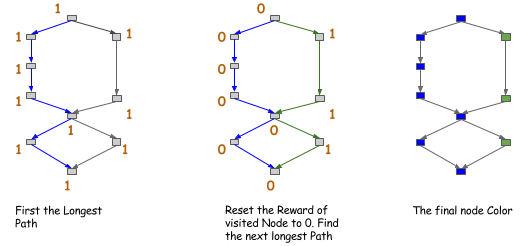
\includegraphics[width=0.95\textwidth]{MXNet/graph_color}
\caption{Color the longest paths in the Graph.}
\end{figure}

After you get the color of the node, you allow sharing (or encourage sharing) only between nodes of the same color. This is a stricter version of the ancestor relationship, but is costs only $O(n)$ of time if you search for only the first $k$ path.

\subsection{How Much Can we Save ?}
On coarse-grained operation graphs that are already optimized for big operations, you can reduce memory consumption roughly by half. You can reduce memory usage even more if you are optimizing a fine-grained computation network used by symbolic libraries, such as Theano.

\subsection{References}
More details can be found in: \href{https://mxnet.incubator.apache.org/architecture/note_memory.html#how-much-can-you-save}{Opimizing the Memory Consumption in DL(MXNet)}.


\section{Deep Learning Programming Style}

Two of the most important high-level design decisions

\begin{itemize}
\item Whether to embrace the symbolic or imperative paradigm for mathematical computation

\item Whether to build networks with bigger or more atomic operations
\end{itemize}

\subsection{Symbolic vs. Imperative Program}

即:符号式编程 vs. 命令式编程

Symbolic programs are a bit different. With symbolic-style programs, we first define a (potentially complex) function abstractly. When defining the function, no actual numerical computation takes place. We define the abstract function in terms of \textbf{placeholder values}(占位符). Then we can compile the function, and evaluate it given real inputs. 

This operation generates a computation graph (also called a symbolic graph) that represents the computation.

Most symbolic-style programs contain, either explicitly or implicitly, a compile step. 

真正的计算只发生在传入数值之时,在这之前,都没有任何计算发生。

The defining characteristic of symbolic programs is their clear separation between building the computation graph and executing it.For neural networks, we typically define the entire model as a single compute graph.

\subsection{Imperative Programs Tend to be More Flexible}

使用命令式编程,那么任何Python语法都可以使用(Nearly anything),但使用符号式编程时,一些Python特性可能无法使用,如迭代。

当使用Python的符号式编程时,实际实在一个Domain-Specific-Language(DSL)定义的空间中进行编程。

Intuitively, you might say that imperative programs are more native than symbolic programs. It’s easier to use native language features. 

\subsection{Symbolic Programs Tend to be More Efficient}

命令式编程与原生Python的相差不大,所以灵活性很高。但符号式编程更有利于速度、存储优化。

Symbolic programs are more restricted. When we call \textit{Compile} on d, we tell the system that only the value of d is needed. The intermediate values of the computation, is then invisible to us.

\begin{itemize}
\item We benefit because the symbolic programs can then safely reuse the memory for in-place computation. 

\item Symbolic programs can also perform another kind of optimization, called operation folding(图\ref{Symbolic1}). In fact, this is one way we hand-craft operations in optimized libraries, such as CXXNet and Caffe. Operation folding improves computation efficiency.

\begin{figure}
\centering
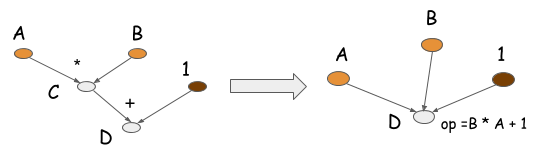
\includegraphics[width=0.75\textwidth]{MXNet/Symbolic1.png}
\caption{Operation Folding示意图。}
\label{Symbolic1}
\end{figure}

Note, you can’t perform operation folding in imperative programs, because the intermediate values might be referenced in the future. Operation folding is possible in symbolic programs because you get the entire computation graph, and a clear specification of which values will be needed and which are not.
\end{itemize}

\subsection{Case Study: Backprop and AutoDiff}
\lstset{language=Python}
\begin{lstlisting}[title=toy model,frame=shadowbox]
import numpy as np
    a = np.ones(10)
    b = np.ones(10) * 2
    c = b * a
    d = c + 1
    ...
\end{lstlisting}


\subsubsection{基于命令式编程的自动求导}
循环调用求导函数,直至最开始的输入变量。

利用grad闭包(Closure)来隐含的保存后向计算图。

但一个坏处是,必须保存所有中间变脸的Grad闭包。

\subsubsection{基于符号式编程的自动求导}

可以实现的优化力度更大。

\subsubsection{Analysis}

可以实现的优化的程度,依赖于可以允许的操作(Restrictions on what you can do)。使用符号式编程时,必须明确提供这些约束,所以可进行优化也就更多。

对于命令式编程,可以通过其它的一些方式添加明确的约束。比如一种方法是Context Variable。如:
\begin{verbatim}
with context.NoGradient()
    ...
\end{verbatim}
可以关闭梯度的计算。但这样也不能利用In-Place Calculation来对存储空间进行复用。

其实是一种trade-off between restriction and flexibility.

\subsection{Model Checkpoint}

保存和加载模型。保存模型的时候,需要保存两类变量:网络的结构配置、网络的权重系数。

符号式编程有利于配置的检查。而对于命令式编程,需要保存所有的代码,或者利用符号式指令进行能够顶层封装。

\begin{itemize}
\item Parameter Updates

大部分符号是编程,都是基于数据流图(Data Flow Graphs, DFG)实现的。DFG描述的是计算。但这种方式下,参数的更新不是很方便。一些做法是将更新过程转化为基于命令式的方式实现,而梯度的计算是基于计算图的方式计算。

\item There is No Strict Boundary

这两种风格的框架其实没有很明显的区分。如在命令式编程时,可以借助Just-in-Time(JIT) Compiler来实现一些符号式编程里面的全局优化等好处。
 
\end{itemize}


\subsection{Big vs. Small Operations}

\begin{itemize}
\item Big Operations

主要是一些经典的神经网络层在用,如Fully Connected and Batch Normalize.

\item Small Operations

一些数学上的计算,如矩阵乘、Element-wise Addition.

\end{itemize}

CXXNet, Caffe支持Layer一级的计算,而Theano, Minerva支持更精细的计算。

\begin{itemize}
\item Smaller Operations Can Be More Flexible (小运算更灵活)

可实现的东西多,且建立新的Layer比较简单,直接添加部件就行。

\item Big Operations Are More Efficient (大运算更高效)

可能引起计算、存储上的开支。

\item Compilation and Optimization

对于小运算的优化,计算图支持一下两种优化:
\begin{itemize}
\item Memory Allocation Optimization

重用中间结果的存储空间。也可用于大运算。

\item Operator Fusion

Fuse several small operations into big one.

\end{itemize}

这些优化对小操作十分重要。小操作对编译器也增加了负担。

\item Expression Template and Statically Typed Language

借助Expression Template来产生具体的Kernels.\href{https://github.com/dmlc/mshadow/blob/master/guide/exp-template/README.md}{Template Expression}, 其实底层是基于C++ Template实现的。

\end{itemize}


\subsection{Mix The Approaches}

Amdahl's Law:
\begin{quote}
 If you are optimizing a non-performance-critical part of your problem, you won’t get much of a performance gain
\end{quote}

实际考虑编程Style时,需要综合考虑:性能、灵活性、工程复杂度等。实践表明,混合使用多个Style可以得到更好的性能。

\begin{itemize}
\item Symbolic and Imperative Programs

有两种方式可以实现这种混用:
\begin{itemize}
\item Use imperative programs within symbolic programs as callbacks
\item Use symbolic programs as part of imperative programs
\end{itemize}
如在参数更新中的讨论。如果代码中,混合了Symbolic和Imperative,那么结果是Imperative.但更好的选择是,用支持GPU计算、参数更新的符号式编程框架来开发。

\item Small and Big Operations
\item Choose Your Own Approach
\end{itemize}

\section{Dependency Engine for Deep Learning}

\subsection{Problems in Dependency Scheduling}

\begin{itemize}
\item Data Flow Dependency

Data flow dependency describes how the outcome of one computation can be used in other computations. 

\item Memory Recycling

\item Random Number Generation

A pseudo-random number generator (PRNG) is not thread-safe because it might cause some internal state to mutate when generating a new number. Even if the PRNG is thread-safe, it is preferable to serialize number generation, so we can get reproducible random numbers.

\end{itemize}

\subsubsection{Design a Generic Dependency Engine}

目标是建立一个轻量级、普用的依赖引擎。目标如下:
\begin{itemize}
\item 识别有效的操作
\item 可以调度GPU、CPU存储的依赖,以及处理随机发生器的依赖
\item 引擎不应分配资源,而仅处理依赖
\end{itemize}

步骤如下:

\begin{enumerate}
\item At the beginning, the user can allocate the variable tag, and attach it to each of the objects that we want to schedule.

\begin{figure}[!hbtp]
\centering
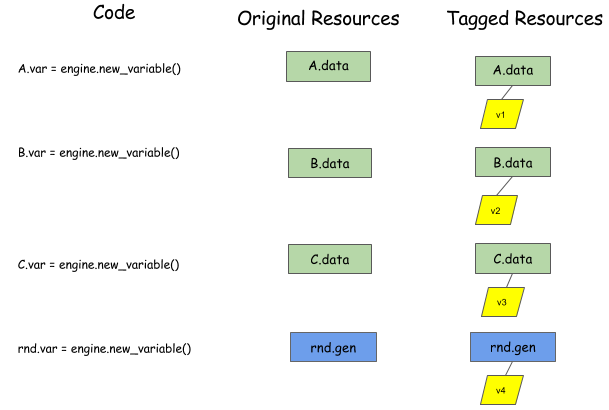
\includegraphics[width=0.75\textwidth]{MXNet/Tag1.png}
\caption{第一步,给变量分配tag}
\label{Tag1}
\end{figure}

\item 然后调用\textit{push}来告知引擎需要运行的函数、参数等,需要区分读取、写入的参数,分别输入。引擎通过识别上一步的tag来识别变量,这样的好处是不涉及tag具体指向什么,所以引擎可以处理包括变量、函数之类的Everything。

\begin{figure}[!hbtp]
\centering
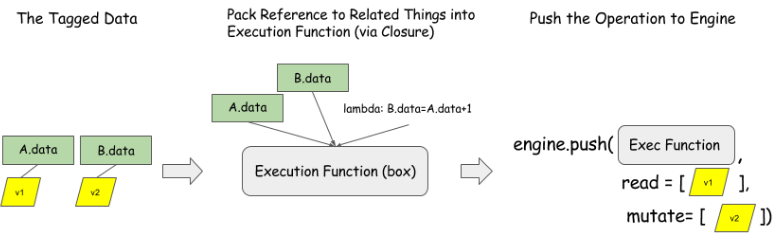
\includegraphics[width=0.75\textwidth]{MXNet/Tag2.png}
\caption{把相应的Function Closure push进依赖分析引擎}
\label{Tag2}
\end{figure}
\end{enumerate}

\subsection{Implementing the Generic Dependency Engine}

基本思想
\begin{itemize}
\item Use a queue to track all of the pending dependencies on each variable tag
\item Use a counter on each operation to track how many dependencies are yet to be fulfilled
\item When operations are completed, update the state of the queue and dependency counters to schedule new operations
\end{itemize}

一个例子如图所示:
\begin{figure}[!hbtp]
\centering
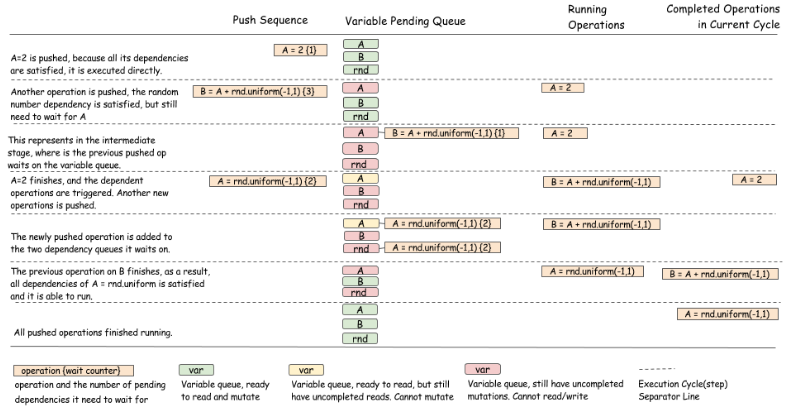
\includegraphics[width=0.95\textwidth]{MXNet/Tag3.png}
\caption{一个具体的例子}
\label{Tag3.png}
\end{figure}

\subsection{Discussion}

\begin{itemize}
\item Dynamic vs. Static
\item Mutation vs. Immutable
\end{itemize}

\section{Designing Efficient Data Loaders for DL}

几点重要的考虑:
\begin{itemize}
\item Small File Size
\item Parallel (Distributed) packing of data
\item Fast data loading and online augmentation
\item Quick reads from arbitrary parts of the dataset in the distributed setting
\end{itemize}

\subsection{Design Insight}

为了设计好的IO系统,需要解决两类任务:Data Preparation, Data Loading.

\subsubsection{Data Preparation}

Data preparation describes the process of packing data into a desired format for later processing. 

\begin{itemize}
\item Pack the dataset into small numbers of files
\item Do the packing once
\item Process the packing in parallel to save time
\item Be able to access arbitrary parts of the data easily
\end{itemize}

\subsubsection{Data Loading}

The next step to consider is how to load the packed data into RAM. 

\begin{itemize}
\item Read Continuously
\item Reduce the bytes to be loaded,可以借助于数据压缩等
\item Load and train in different threads
\item Save RAM
\end{itemize}

\subsection{Data Format}

需要选择既高效又方便的数据结构。为了实现这个目标,把二进制数据包装成可以分离的结构。具体,MXNet采用DMLC-Core里面的recordIO类型。

\begin{figure}[!hbtp]
\centering
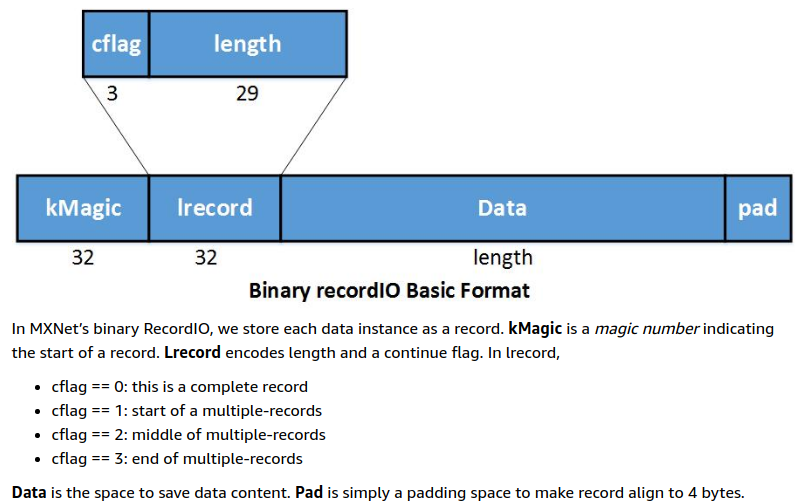
\includegraphics[width=0.95\textwidth]{MXNet/recordIO1.png}
\caption{Binary recordIO数据结构}
\label{recordIO1}
\end{figure}

通过连续读,来避免随机读引入的延时。

这种数据结构的一个好处是,每一个record的长度可以改变。从而支持更好的数据压缩。

\begin{figure}[!hbtp]
\centering
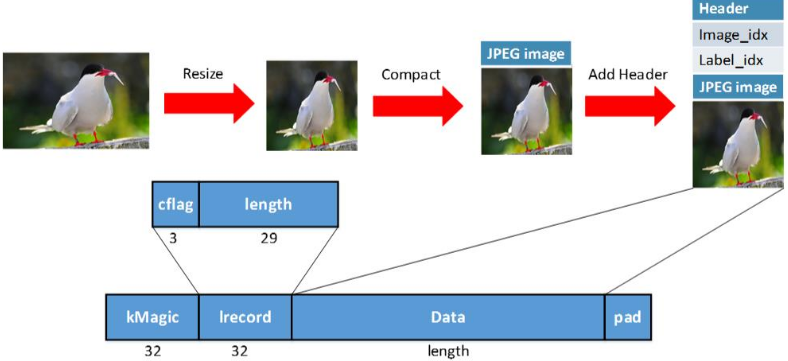
\includegraphics[width=0.95\textwidth]{MXNet/recordIO2.png}
\caption{Binary recordIO的一个例子}
\label{recordIO2}
\end{figure}
其中,\textit{resize}把输入图像变为256 * 256大小。


\subsubsection{Access Arbitrary Parts of Data}

The packed data can be logically sliced into an arbitrary number of partitions, no matter how many physical packed data files there are.

在recordIO中借助Magic Number来实现上述目的,具体是使用dmlc-core中的\textit{InputSplit}函数来实现。这个函数极大的帮助了并行实现,因为每一个节点只处理一个\textit{Part}.

\subsection{Data Loading and Preprocessing}

\subsubsection{Loading and Preprocessing on the Fly}

In service of efficiency, we also address multi-threading techniques. 

\begin{figure}[!hbtp]
\centering
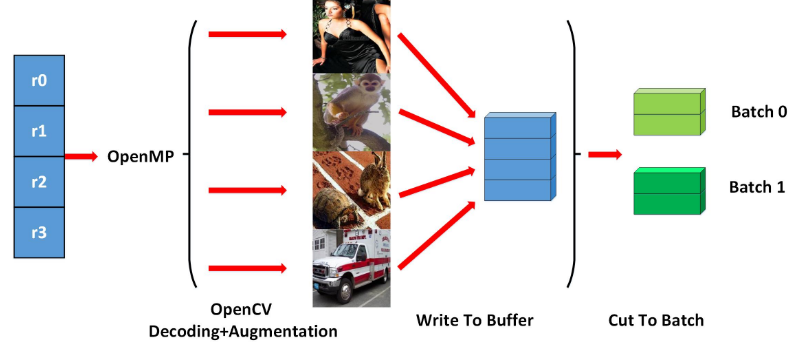
\includegraphics[width=0.95\textwidth]{MXNet/loadingData1.png}
\caption{并行预处理例子}
\label{loadingData1}
\end{figure}

在加载了大量图像数据后,利用多线程工具(OpenMP)进行并行处理。

\subsubsection{Hide IO Cost Using Threadediter}

一种降低IO影响的办法是:数据预取。具体使用dmlc-core提供的\textit{threadediter}来处理IO. The key of threadediter is to start a stand-alone thread that acts as a data provider, while the main thread acts as a data consumer as illustrated below.

The threadediter maintains a buffer of a certain size and automatically fills the buffer when it’s not full. And after the consumer finishes consuming part of the data in the buffer, threadediter will reuse the space to save the next part of data. 

\begin{figure}[!hbtp]
\centering
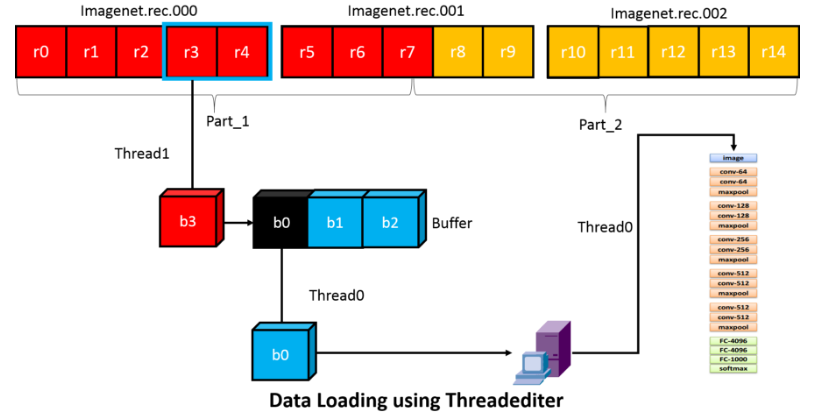
\includegraphics[width=0.95\textwidth]{MXNet/dataLoading2.png}
\caption{数据预取的示意图,借助Buffer来实现}
\label{loadingData2}
\end{figure}


\subsection{MXNet IO Python Interface}

We make the IO object as an iterator in numpy. By achieving that, the user can easily access the data using a for-loop or calling next() function. Defining a data iterator is very similar to defining a symbolic operator in MXNet.

为了创建一个数据迭代器,需要提供五种类型的参数:

\begin{itemize}
\item Dataset Param: 如路径、输入的尺寸等
\item Batch Param: Batch Size
\item Augmentation Param: 确定数据增广的类型,如翻转等
\item Backedn Param:  控制后台线程,来隐藏数据读取延时
\item Auxiliary Param: 帮助Debug的信息等。
\end{itemize}

通常必须确定\textbf{Dataset Param}和\textbf{Batch Param}。MX Data IO也支持模块化,如以下两种:
\begin{itemize}
\item 自己的高效数据预取。allows the user to write a data loader that reads their customized binary format that automatically gets multi-threaded prefetcher support.

\item 数据转换。image random cropping, mirroring, etc. Allows the users to use those tools, or plug in their own customized transformers

\end{itemize}


\section{Except Handling in MXNet}

MXNet在两类情况下可以抛出异常:
\begin{itemize}
\item MXNet main thread. For \textit{e.g.} Infershape and InferType。 在主线程中处理
\item Spawned threads (生成线程?)
\begin{itemize}
\item By dependency engine for operator execution in parallel。会被rethrown到主线程,进行处理
\item By the iterators, during the data loading, text parsing phase \textit{etc.}
\end{itemize}
\end{itemize}

\subsubsection{Exception Handling for Iterators}

CVIter 使用 PrefetcherIter来加载和解析数据。PrefetcherIter会生成一个Producer线程并后台运行,在主线程(Consumer)中使用这些数据。在Producer线程中可能抛出异常,该异常被发送到主线程。


可能引起线程之间的竞争(Race).To avoid this situation, you should try and iterate through your full dataset if you think it can throw exceptions which need to be handled.

\subsubsection{Except Handling for Operators}

For the operator case, the dependency engine spawns a number of threads if it is running in the \textbf{ThreadedEnginePool} or \textbf{ThreadedEnginePerDevice} mode. The final operator is executed in one of the spawned threads.

If an operator throws an exception during execution, this exception is propagated down the dependency chain. Once there is a synchronizing call i.e. \textbf{WaitToRead} for a variable in the dependency chain, the propagated exception is rethrown.


\textbf{注意}:Please avoid waitalls in your code unless you are confident about your code not throwing exception in any scenario. 因为\textbf{mx.nd.waitall}不支持rethrowing异常。

\section{MXNet-Gluon创建模型}

参考文献:\href{zh.gluon.ai}{Gluon}

\subsection{模型构造}

继承\verb|gluon.nn.Block|来实现,必须重载\verb|forward|函数。在\verb|__init__|函数里面定义模型所需的变量等。

\textbf{需要值得注意的地方是},在基于自定义的模型构建大的模型时,需要调用的是\verb|__init__|函数的参数;而一旦模型定义好了,开始向里面传入数据时,数据的格式需要根据\verb|forward|函数来确定!

\subsubsection{两种稍微不同的实现}
方式一,是直接利用Gluon预定义的层构建类型变量。
\lstset{language=Python, caption={自定义模型,方式一}, label=MXNetModel0}
\begin{lstlisting}
from mxnet import nd
from mxnet.gluon import nn

class MLP(nn.Block):
    # 声明带有模型参数的层,这里我们声明了两个全链接层。
    def __init__(self, **kwargs):
        # 调用 MLP 父类 Block 的构造函数来进行必要的初始化。这样在构造实例时还可以指定
        # 其他函数参数,例如下下一节将介绍的模型参数 params。
        super(MLP, self).__init__(**kwargs)
        # 隐藏层。
        self.hidden = nn.Dense(256, activation='relu')
        # 输出层。
        self.output = nn.Dense(10)
    # 定义模型的前向计算,即如何根据输出计算输出。
    def forward(self, x):
        return self.output(self.hidden(x))
\end{lstlisting}

方式二,即先定义一个Sequential的类型变量Net,然后在向里面增加\verb|gluon.nn.Layer|等具体的层,或者自己定义的层。
\lstset{language=Python, caption={自定义模型,方式二}, label=MXNetModel1}
\begin{lstlisting}
class NestMLP(nn.Block):
    def __init__(self, **kwargs):
        super(NestMLP, self).__init__(**kwargs)
        self.net = nn.Sequential()
        self.net.add(nn.Dense(64, activation='relu'),
                     nn.Dense(32, activation='relu'))
        self.dense = nn.Dense(16, activation='relu')

    def forward(self, x):
        return self.dense(self.net(x))  #调用要加self

net = nn.Sequential()
net.add(NestMLP(), nn.Dense(20), FancyMLP())

net.initialize()
net(x)
\end{lstlisting}

由于FancyMLP和Sequential都是Block的子类,我们可以嵌套调用他们。

实际使用中,貌似还存在第三种构建方式,直接以函数的形式使用, 如VGG:
\lstset{language=Python, caption={自定义模型VGG11,方式三}, label=MXNetLayer2}
\begin{lstlisting}
import sys
sys.path.append('..')
import gluonbook as gb
from mxnet import nd, init, gluon
from mxnet.gluon import nn

def vgg_block(num_convs, num_channels):
    blk = nn.Sequential()
    for _ in range(num_convs):
        blk.add(nn.Conv2D(
            num_channels, kernel_size=3, padding=1, activation='relu'))
    blk.add(nn.MaxPool2D(pool_size=2, strides=2))
    return blk
conv_arch = ((1,64), (1,128), (2,256), (2,512), (2,512))

def vgg(conv_arch):
    net = nn.Sequential()
    # 卷积层部分
    for (num_convs, num_channels) in conv_arch:
        net.add(vgg_block(num_convs, num_channels))
    # 全连接层部分
    net.add(nn.Dense(4096, activation="relu"), nn.Dropout(.5),
            nn.Dense(4096, activation="relu"), nn.Dropout(.5),
            nn.Dense(10))
    return net

net = vgg(conv_arch)
\end{lstlisting}

\subsection{自定义层}

也需要继承\verb|gluon.nn.Block|以及重载\verb|forward|函数。

\lstset{language=Python, caption={自定义层,方式一}, label=MXNetLayer0}
\begin{lstlisting}
class CenteredLayer(nn.Block):
    def __init__(self, **kwargs):
        super(CenteredLayer, self).__init__(**kwargs)

    def forward(self, x):
        return x - x.mean()
\end{lstlisting}

\subsubsection{带参数的自定义层}

我们还可以自定义含模型参数的自定义层。这样,自定义层里的模型参数就可以通过训练学出来了。我们在“模型参数”一节里介绍了Parameter类。其实,在自定义层的时候我们还可以使用Block自带的ParameterDict类型的成员变量params。顾名思义,这是一个由字符串类型的参数名字映射到Parameter类型的模型参数的字典。我们可以通过get函数从ParameterDict创建Parameter,注意是创建,也就是加入!

\lstset{language=Python, caption={带参数的自定义层,方式一}, label=MXNetLayer1}
\begin{lstlisting}
class MyDense(nn.Block):
    def __init__(self, units, in_units, **kwargs):
        super(MyDense, self).__init__(**kwargs)
        self.weight = self.params.get('weight', shape=(in_units, units))
        self.bias = self.params.get('bias', shape=(units,))

    def forward(self, x):
        linear = nd.dot(x, self.weight.data()) + self.bias.data()
        return nd.relu(linear)
\end{lstlisting}

\subsection{实际例子}

\subsubsection{ResNet}

使用的是自定义层方式一中的方式构建残差块。然后定义更高一级的结构(自定义模型方式二中的方法),最后再在更高一级进行构架整个模型。层次结构如下:

\lstset{language=Python, caption={ResNet using Gluon}}
\begin{lstlisting}
import sys
sys.path.append('..')
import gluonbook as gb
from mxnet import nd, gluon, init
from mxnet.gluon import nn

# 构建底层
class Residual(nn.Block):
    def __init__(self, num_channels, use_1x1conv=False, strides=1, **kwargs):
        super(Residual, self).__init__(**kwargs)
        self.conv1 = nn.Conv2D(num_channels, kernel_size=3, padding=1,
                               strides=strides)
        self.conv2 = nn.Conv2D(num_channels, kernel_size=3, padding=1)
        if use_1x1conv:
            self.conv3 = nn.Conv2D(num_channels, kernel_size=1,
                                   strides=strides)
        else:
            self.conv3 = None
        self.bn1 = nn.BatchNorm()
        self.bn2 = nn.BatchNorm()

    def forward(self, X):
        Y = nd.relu(self.bn1(self.conv1(X)))
        Y = self.bn2(self.conv2(Y))
        if self.conv3:
            X = self.conv3(X)
        return nd.relu(Y + X)

# 构建高一层        
def resnet_block(num_channels, num_residuals, first_block=False):
    blk = nn.Sequential()
    for i in range(num_residuals):
        if i == 0 and not first_block:
            blk.add(Residual(num_channels, use_1x1conv=True, strides=2))
        else:
            blk.add(Residual(num_channels))
    return blk
    
# 构建整个模型
net.add(resnet_block(64, 2, first_block=True),
        resnet_block(128, 2),
        resnet_block(256, 2),
        resnet_block(512, 2))        
\end{lstlisting}

需要注意的是,即使在\verb|class|里面也可以调用底层的自定义模块,如在\verb|resnet_block|中调用\verb|Residual|,具体调用方式是调用底层类的构造函数,即\verb|__init__|函数,参数要跟这个函数的参数一致。

\subsubsection{DenseNet}

发现与上面的ResNet类似,所以这里省略。

\section{MXNet中的Deconvolution}

具体实现是, \verb|Conv2DTranspose|等。

由于\verb|Conv2DTranspose|这个函数回引起棋盘状 Artifacts,所以在MXNet里面,还有一个上采样卷积的函数:\verb|mxnet.ndarray.UpSampling()|, \textbf{但是}, 听说目前还不好用啊。

参考\href{https://discuss.gluon.ai/t/topic/3041/14}{FCN讨论区-chen0510566}回答,\verb|gluon.nn.Conv2DTranspose|的文档,\verb|Conv2DTranspose|输出的size是这样计算的:
\begin{displaymath}
\begin{gathered}
Out\_height = (height - 1) * strides[0] - 2 * padding[0] + kernel\_size[0] + output\_padding[0] \\
Out\_width = (width - 1) * strides[1] - 2 * padding[1] + kernel\_size[1] + output\_padding[1]
\end{gathered}
\end{displaymath}

$\uparrow$正确性有待验证。

\section{MXNet读取训练数据}

重要,我发现,对于我这样的新手来说,如何处理数据也是个问题,尤其现在,我感觉一头雾水。

参考文章:

[1] \href{https://www.jianshu.com/p/38d55c9dbdb8}{MXNet常见加载数据的方式-简书}

[2] \href{https://mxnet.incubator.apache.org/api/python/io/io.html}{MXNet API}


有必要对MXNet的数据结构进行说明一下!尤其对于axes的概念。在MXNet中,我认为axes可以取四个值,分别对应以下概念:
\begin{itemize}
\item axes = 0, Batches, 比如batchsize=8, 那么axes就对应这8个样本
\item axes = 1, Channels, 比如输入彩色图像,那么axes对应的就是RGB三个通道
\item axes = 2, Width or Height, 还不太确定,与axes=3共同确定每一个Channel的尺寸
\end{itemize}

接下来就是本小节的重点内容,也就是如果处理训练数据,这是开始的一步,但我感觉也是容易被各种教程忽视的一步,如果这步不清楚,那么会影响整个后面的学习与实践过程。

{\bfseries 正如参考文献中所总结的那样,一共可以分为三类。分别如下!}

\begin{itemize}
\item 基于mxnet.io读取数据
\item 使用mxnet.iamge读取数据
\item \textbf{使用gluon接口读取数据}, 这个部分是重点
\end{itemize}

此外,作者还提到了几种支持的数据结构,貌似就这几种么?
\begin{itemize}
\item .rec文件
\item raw image
\item .lst文件,使用mx.image.ImageIter接口读取,这个接口可以读.rec的文件
\end{itemize}

大概流程:传data iter对象给base\_module,把数据对象变为iterator。
下面分别对三种数据读取方式进行示例。

\subsection{使用mx.io读取数据}

\subsubsection{从内存中读取}

调用\verb|mx.io.NDArrayIter|接口,以MXNet官方的train\_mnist.py为例。

\lstset{language=Python, caption={train\_mnist.py例子}}
\begin{lstlisting}
def read_data(label, image):
   """
   download and read data into numpy
   """
   base_url = 'http://yann.lecun.com/exdb/mnist/'
   with gzip.open(download_file(base_url+label, os.path.join('data',label))) as flbl:
       magic, num = struct.unpack(">II", flbl.read(8))
       label = np.fromstring(flbl.read(), dtype=np.int8)
   with gzip.open(download_file(base_url+image, os.path.join('data',image)), 'rb') as fimg:
       magic, num, rows, cols = struct.unpack(">IIII", fimg.read(16))
       image = np.fromstring(fimg.read(), dtype=np.uint8).reshape(len(label), rows, cols)
   return (label, image)


def to4d(img):
   """
   reshape to 4D arrays
   """
   return img.reshape(img.shape[0], 1, 28, 28).astype(np.float32)/255

def get_mnist_iter(args, kv):
   """
   create data iterator with NDArrayIter
   """
   (train_lbl, train_img) = read_data(
           'train-labels-idx1-ubyte.gz', 'train-images-idx3-ubyte.gz')
   (val_lbl, val_img) = read_data(
           't10k-labels-idx1-ubyte.gz', 't10k-images-idx3-ubyte.gz')
   train = mx.io.NDArrayIter(
       to4d(train_img), train_lbl, args.batch_size, shuffle=True)
   val = mx.io.NDArrayIter(
       to4d(val_img), val_lbl, args.batch_size)
   return (train, val)
#参考train_mnist.py
\end{lstlisting}

详解如下:
\begin{itemize}
\item 顶层函数为\verb|get_mnist_iter|函数

该函数的参数是:包含batch size的类arg。kv参数,但貌似没用到。

函数\verb|get_mnist_iter|调用\verb|read_data|函数,返回图像数据及其对应的label。该函数的

将\verb|read_data|函数的返回值传入\verb|mx.io.NDArrayIter|函数,该函数返回名称为\verb|train|和\verb|val|的data iterator. 分别作用与训练图像与训练标签。\verb|NDAarrayIter|函数的使用参数解释在下文单独总结。

返回data iterator的训练图像与训练标签。

\item 被调用函数\verb|read_data|

该函数在这里主要负责下载数据文件(download\_file())、解压缩(struct.unpack)等。各个函数的输入输出可参考源代码。

\item 被调用函数\verb|to4d|

负责把输入图片rehape成四维数据结构,维度分解见上文中的axes的解释。

\end{itemize}

所以总结一下的话,就是这样的,首先下载文件并解压缩,然后读取数据,送入\verb|mx.io.NDArrayIter|产生data iterator.

\subsubsection{从.csv文件中读取数据}

\lstset{language=Python, caption={Read .csv 数据}}
\begin{lstlisting}
#lets save `data` into a csv file first and try reading it back
np.savetxt('data.csv', data, delimiter=',')
data_iter = mx.io.CSVIter(data_csv='data.csv', data_shape=(3,), batch_size=30)
for batch in data_iter:
   print([batch.data, batch.pad])
\end{lstlisting}

详解:
\begin{itemize}
\item 调用\verb|mx.io.CSVIter|读取.csv格式文件,同时输入数据shape以及batch size。返回的就是一个 data iterator。
\end{itemize}

\subsubsection{使用mx.io.ImageRecordIter接口,需要定制KVStore}

这一部分还没看明白,可以看一下原文。

\subsection{常用的系统提供的接口函数}
分析以上实现方式,主要涉及以下几个系统接口函数。
\begin{itemize}
\item \verb|mx.io.NDArrayIter|

原型:class mxnet.io.NDArrayIter(data, label=None, batch\_size=1, shuffle=False, last\_batch\_handle='pad', data\_name='data', label\_name='softmax\_label')

其中,data, label为array 或list of array or dict of string to array。

last\_batch\_handle为最后一个batch的处理,即训练数据的数目不能被batch size整除时的处理方式,可以选取'pad', 'discard' or 'roll\_over'等。

更多细节见文档吧。

Returns an iterator for mx.nd.NDArray, numpy.ndarray, h5py.Dataset mx.nd.sparse.CSRNDArray or scipy.sparse.csr\_matrix.


\item \verb|mx.io.CSVIter|

return the CSV file iterator,详情见文档吧。

\item \verb|struct.unpack|

原型:\verb|struct.unpack(fmt, buffer)|

Unpack from the buffer buffer (presumably packed by pack(fmt, ...)) according to the format string fmt. The result is a tuple even if it contains exactly one item. The buffer’s size in bytes must match the size required by the format, as reflected by calcsize().关于fmt的具体格式,参考\href{https://docs.python.org/3/library/struct.html}{struct library python}

\item \verb|gzip.read()|

原型:\verb|read(size=-1)|

Read and return up to size bytes. If the argument is omitted, None, or negative, data is read and returned until EOF is reached. An empty bytes object is returned if the stream is already at EOF.

If the argument is positive, and the underlying raw stream is not interactive, multiple raw reads may be issued to satisfy the byte count (unless EOF is reached first). But for interactive raw streams, at most one raw read will be issued, and a short result does not imply that EOF is imminent.

所以参数是要读取的byte的数目。

\end{itemize}

\subsection{使用mx.image读取数据}

从imagelist中读取可迭代的数据。

\lstset{language=Python, caption={mx.image使用示例}}
\begin{lstlisting}
data_iter = mx.image.ImageIter(batch_size=4, data_shape=(3, 224, 224), label_width=1,
data_iter.reset()
for data in data_iter:
d = data.data[0]
print(d.shape)
# we can apply lots of augmentations as well
data_iter = mx.image.ImageIter(4, (3, 224, 224), path_imglist='data/custom.lst',
data = data_iter.next()
# specify augmenters manually is also supported
data_iter = mx.image.ImageIter(32, (3, 224, 224), path_rec='data/caltech.rec',
\end{lstlisting}

详解:
\begin{itemize}
\item 调用\verb|mx.image.ImageIter|实现
\end{itemize}

\subsection{使用Gluon接口读取数据}

由于用的比较多,所以这部分是重点,起码目前来看是重点。

使用Gluon接口时,我觉着主要分为两步:产生Dataset,基于Dataset产生 Mini-batch iterator!

下面分别对这两个步骤进行简单说明,后续有时间在详细说一下吧。通过本小节的简单解释,然后再看这个文档,应该就不那么难了吧,就知道各个部分是什么意思了,怎么组织在一起的了。

具体的参考文档:\href{https://mxnet.incubator.apache.org/api/python/gluon/data.html}{Gluon API 文档}

\subsubsection{产生Dataset}

Dataset的生成主要分为几种方式,这里主要讨论三种形式:
\begin{itemize}
\item Gluon自带的数据库,包括:MNIST, FashionMNIST, CIFAR10, CIFAR100等。

产生Dataset的方式为:

\begin{verbatim}
data_set = gluon.data.vision.Dataset
\end{verbatim}

其中, Dataset需要替换成提到的提供的自带数据库。

\item 来自目录生成Dataset, 调用:\verb|ImageFolderDataset|, 目录中保存的raw image。

产生Dataset的方式:

\begin{verbatim}
data_set = gluon.data.vision.ImageFolderDataset(root, flag=1, tranform=None)
\end{verbatim}

A dataset for loading image files stored in a folder structure like:看文档,ImageFolderDataset的说明文档。其中,flag=1说明把读入的图像转换成三通道彩色的,若flag=0那么读入的是灰度图像。

\item 自己生成Dataset类!

产生自定义Dataset的方式:

\begin{verbatim}
class myDatasetName(gluon.data.Dataset)
    ... other functions, to process image as your need
    def __getitem__(..):
        ....
    def __len__(..):
        ....
\end{verbatim}

从上面的代码可以看出,生成自定义的Dataset时,需要继承\verb|gluon.data.Dataset|类,同时,必须override \verb|__getitem__|和\verb|__len__|两个函数!实际使用中,该类可以按照自己数据库的格式,在myDatasetName类中定义其它帮助处理数据的函数,一个更具体点的例子是\href{http://zh.gluon.ai/chapter_computer-vision/fcn.html}{FCN-Gluon}这个文档的代码!

\end{itemize}

\subsubsection{产生Mini-batch iterator}

在上一步,\textbf{无论用哪一种方式}产生了Dataset后,就可以送入\verb|DataLoader|产生data iterator了!

这一步主要通过借助\verb|gluon.data.Dataloader|这一Iterator类来实现。此外还有一些基于Sample的函数,具体看文档。

产生Mini-batch Iterator的方式:

\begin{verbatim}
data_iter = gluon.data.DataLoader(dataset, batch_size=Noen,  
                                          shuffle=False, ....)
\end{verbatim}

后面还有很多参数,可以去文档查看。

这里的第一个参数:\verb|dataset|也就是上文提到的生成Dataset的结果了。

\section{Gluon中的数据结构}

这一部分,我主要想总结一下Gluon中的各种部件的数据结构,如Net = gluon.nn.Sequentional()后,net的数据结构到底是什么样的,还有就是网络的参数又是什么结构的, 比如Parameter类到底长什么样,又该如何使用等。有时间慢慢写吧。









